%!TEX program = xelatex
\documentclass[cn,hazy,pku,12pt,normal,math=newtx,cite=super]{elegantnote}
\title{稀溶液法测定极性分子的偶极矩}

\author{刘松瑞 \quad 2100011819 \\ 组号:24 \quad 组内编号:5}
\institute{化学与分子工程学院}

\expdate{\zhdate{2023/12/14}}
\temperature{18.0 \si{^{\circ}C}}
\pressure{102.21 \si{kPa}}

\usepackage{gensymb}
\usepackage{array}
\usepackage{subfigure}
\usepackage[fontset=windows]{ctex}
\usepackage{graphicx}
\usepackage{float}
\usepackage{caption}
\usepackage{multirow}
%\usepackage{subfig}
%\usepackage{float}
\begin{document}

\maketitle

\abstracts{
    本实验通过稀溶液法测定正丁醇的偶极矩,通过测定密度和电容,
求出其总摩尔极化度为 $(8.5 \pm 0.6) \times 10^{-5}m^3/mol$;
利用阿贝折射仪测定正丁醇的折射率,进而求出其电子极化度
也就是摩尔折射度为 $(2.2281 \pm 0.0007) \times 10^{-5} m^2\cdot mol^{-1}$。
进一步计算其偶极矩为 $(1.72 \pm 0.08) D$。实验的误差主要来自于电容的测量和实验的原理误差,可以通过减小
实验体系的浓度,维持实验温度为一定值,来提高偶极矩的测量准确性。
}
\keywords{
    偶极矩\quad 正丁醇\quad 介电常数\quad 折射率
}

\newpage


\section{引言}

\subsection{实验目的、原理与方法}
实验目的、原理与方法详见预习报告图~\ref{1}。 \cite{pcl2002}

\begin{figure}[htbp]
    \centering
    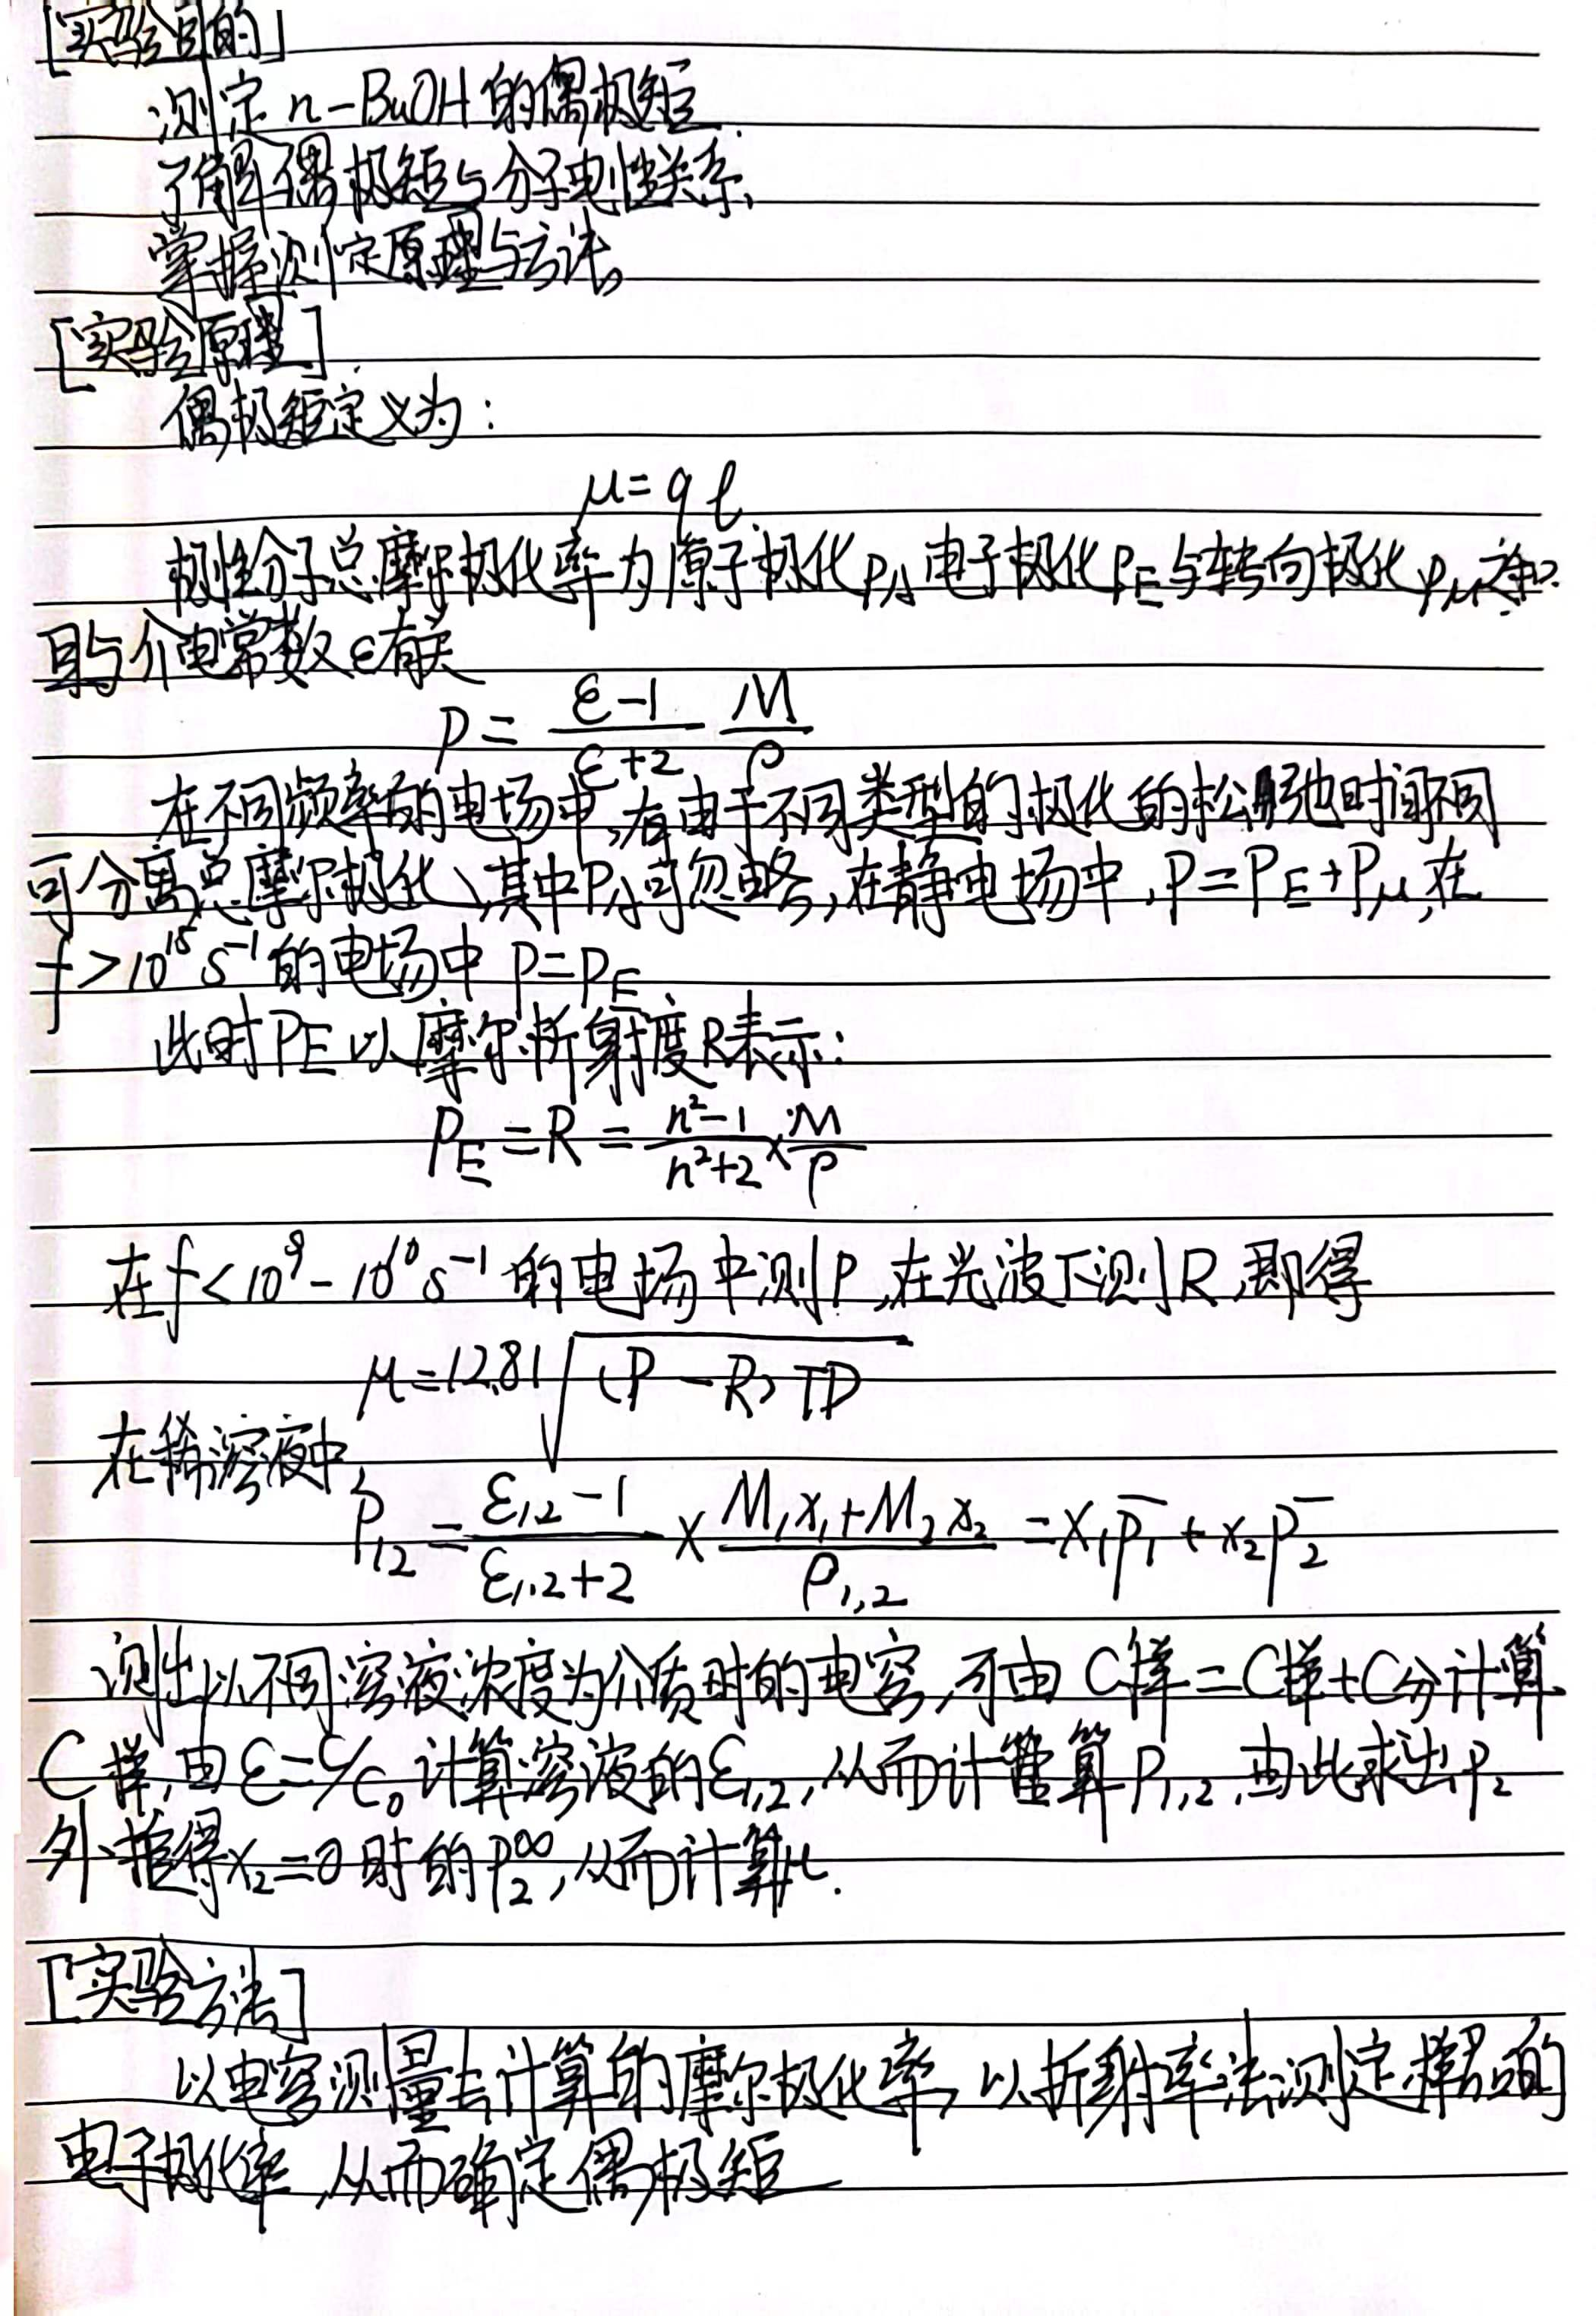
\includegraphics[width = .70\textwidth]{image/yxbg_1.jpg}
    \caption{实验的目的与原理}\label{1}
\end{figure}

\section{实验部分}

\subsection{实验步骤}
实验步骤详见预习报告图~\ref{2}。

\begin{figure}[htbp]
    \centering
    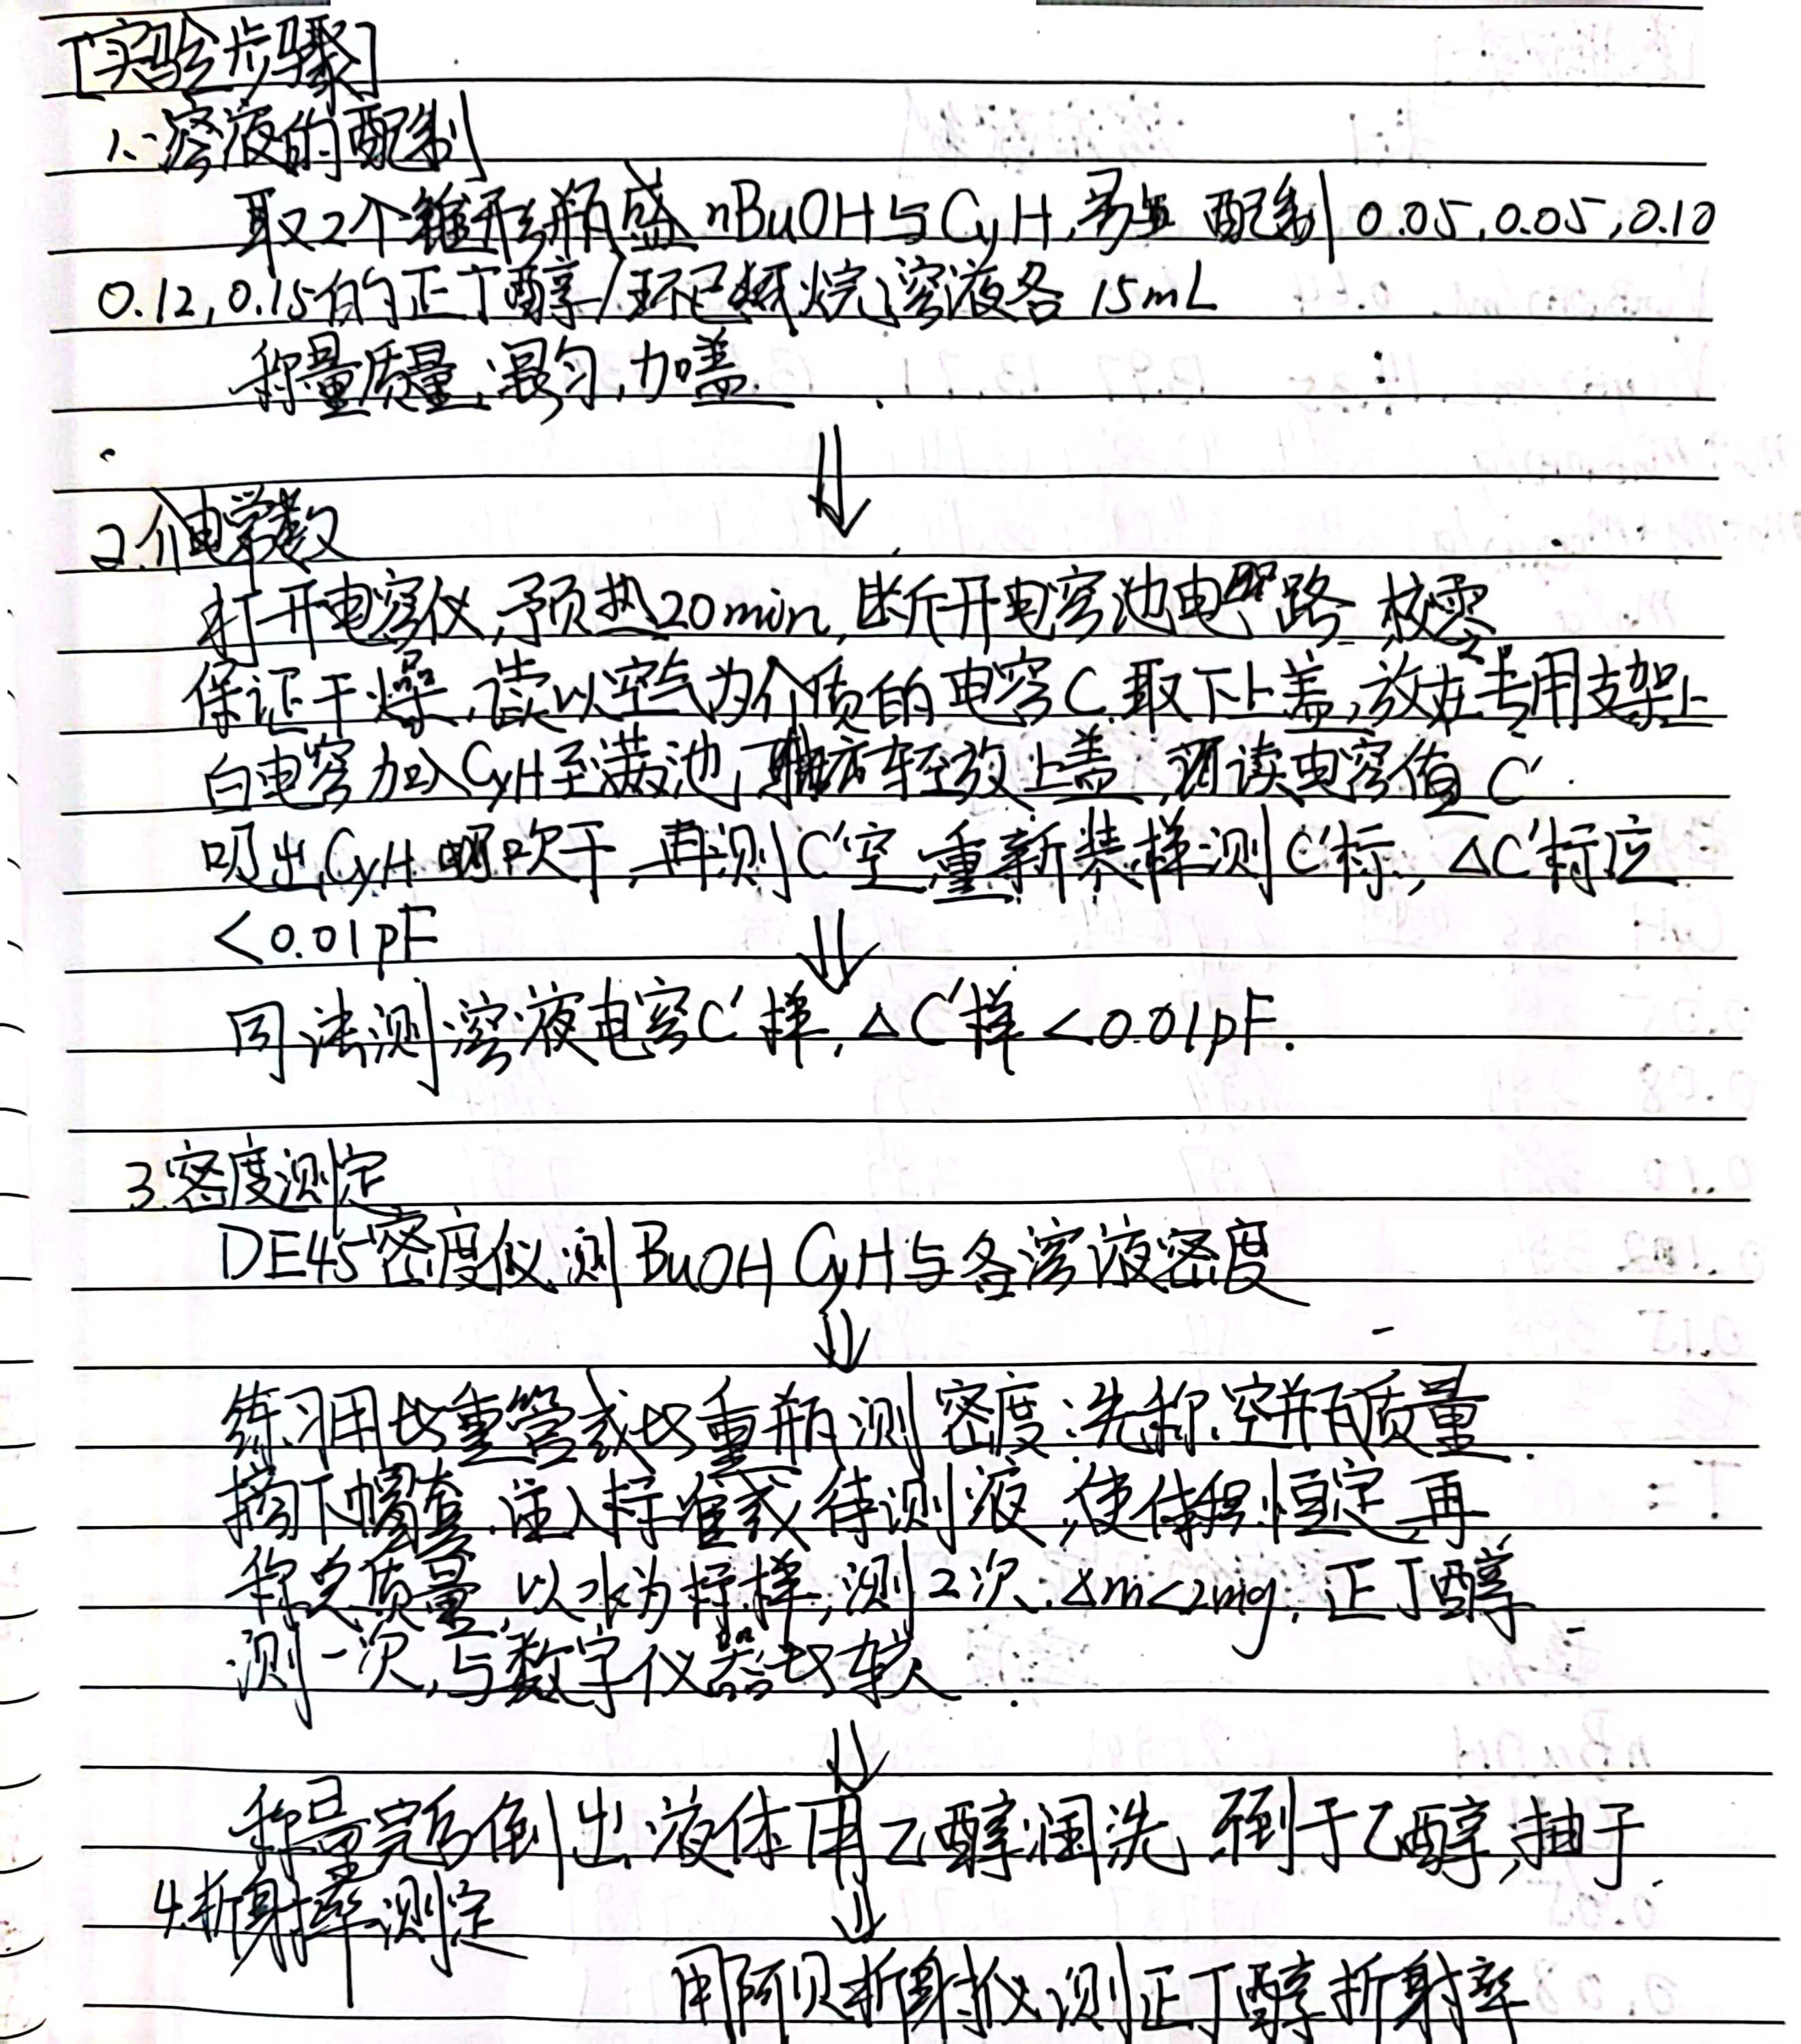
\includegraphics[width = .70\textwidth]{image/yxbg_2.jpg}
    \caption{实验的目的与原理}\label{2}
\end{figure}

\subsection{仪器与药品}

\begin{enumerate} %有序列表
    \item 试剂 \\   正丁醇,环己烷,丙酮,乙醇。
    \item 仪器 \\   PCM-1 型精密电容测量仪,电容池,注射器,洗耳球,50 mL 磨口锥形瓶(7 个),
    滴管,吸量管,烧杯(50 mL,200 mL 各 1 个),电子天平,阿贝折射仪,循环水真空泵,DE45 型数字密度计,
    D50 型数字密度计。
\end{enumerate}

\section{实验现象与数据处理}

\subsection{溶液配制}

配置不同浓度的正丁醇溶液,实验记录空瓶重,加入正丁醇的瓶重与加入正丁醇与环己烷的瓶重。可以计算
瓶中正丁醇与环己烷的重量与正丁醇摩尔分数,列于表 \ref{01} 中
\begin{equation}
 x = \frac{m_{BuOH}/M_{BuOH}}{m_{BuOH}/M_{BuOH}+m_{CyH}/M_{CyH}}    
\end{equation}


\begin{table}[h]
    \centering
    \caption{称量数据和各溶液的摩尔分数}
    \label{01}
    \begin{tabular}{cccccc}
    \hline
    $x_0$ & $V_{BuOH}$ & $V_{CyH}$ & $m_{BuOH}$ & $m_{CyH}$ & $x$   \\ \hline
    0.05  & 0.64       & 14.35     & 0.590      & 13.710    & 0.049 \\
    0.08  & 1.03       & 13.97     & 0.950      & 12.940    & 0.078 \\
    0.10  & 1.29       & 13.71     & 1.190      & 12.420    & 0.098 \\
    0.12  & 1.55       & 13.45     & 1.430      & 11.900    & 0.117 \\
    0.15  & 1.95       & 13.05     & 1.800      & 11.100    & 0.149 \\ \hline
    \end{tabular}
\end{table}


\subsection{电容测量与介电常数计算}

通过实验测得电容的实验数据列于表 \ref{02} 。

\begin{table}[h]
    \centering
    \caption{以不同物质为介质的电容数值}
    \label{02}
    \begin{tabular}{cccccc}
    \hline
    $x$   & $C_0'/pF$ & $C_{sample}'/pF$ & $C_0'/pF$  & $C_{sample}'/pF$ & $\overline{C_{sample}'}/pF$       \\ \hline
    0.000 & 3.99     & 6.56            & 3.99       & 6.56             & 6.56                   \\
    0.049 & 3.99     & 6.77            & 3.99       & 6.77             & 6.77                   \\
    0.078 & 3.99     & 6.94            & 3.99       & 6.94             & 6.94                   \\
    0.098 & 3.99     & 7.07            & 3.99       & 7.07             & 7.07                   \\
    0.117 & 3.99     & 7.20            & 3.99       & 7.20             & 7.20                   \\
    0.149 & 3.99     & 7.54            & 3.99       & 7.54             & 7.54                   \\ \hline
    \end{tabular}       
\end{table}

环己烷的相对介电常数可以由经验公式给出,并将其作为标准介电常数
\begin{equation}
    \varepsilon_{CyH} =  2.023 - 0.0016 ( T - 293 ) = 2.026\ pF = \varepsilon_{standard}
\end{equation}

实测平均空气电容可以计算得到
$$
C_{air}'= \bar{C_0'} = 3.99\ pF
$$

分布电容为
\begin{equation}
    C_{d} = C_{air}'-\frac{\overline{C_{standard}'}-C_{air}'}{\varepsilon_{standard} - 1} =\ 1.49 pF
\end{equation}
又由于
\begin{equation}\label{001}
    C_{sample} = \overline{C_{sample}'}-C_d
\end{equation}
由公式\ref{001},可以推导
\begin{equation}
    \varepsilon = \frac{C_{sample}}{C_{air}} = \frac{\overline{C_{sample}'}-C_d}{C_{air}' - C_d}
\end{equation}

可以计算各个溶液的相对介电常数,如表 \ref{03} 所示。

\begin{table}[h]
    \centering
    \caption{以不同物质为介质的介电常数}
    \label{03}
    \begin{tabular}{cc}
    \hline
    $x$   & $\varepsilon$ \\ \hline
    0.000 & 2.0262        \\
    0.049 & 2.110053      \\
    0.078 & 2.177934      \\
    0.098 & 2.229843      \\
    0.117 & 2.281752      \\
    0.149 & 2.417514      \\ \hline
    \end{tabular}
\end{table}

\subsection{密度测量}

\begin{table}[h]
    \centering
    \caption{环己烷、正丁醇和不同浓度溶液的密度}
    \label{04}
    \begin{tabular}{ccccc}
    \hline
    $x$ & \multicolumn{3}{c}{$\rho$/$\rm g\cdot   cm^{-3}$} & \multicolumn{1}{c}{$\bar{\rho}$/$\rm g\cdot cm^{-3}$} \\ \hline
    0.000 & 0.7784  & 0.7784  & 0.7784  & 0.7784  \\
    0.049 & 0.7787  & 0.7787  & 0.7787  & 0.7787  \\
    0.078 & 0.7791  & 0.7791  & 0.7791  & 0.7791  \\
    0.098 & 0.7794  & 0.7795  & 0.7795  & 0.7795  \\
    0.117 & 0.7797  & 0.7798  & 0.7798  & 0.7798  \\
    0.149 & 0.7803  & 0.7804  & 0.7804  & 0.7804  \\
    1.000 & 0.80945 & 0.80945 & 0.80944 & 0.80945 \\ \hline
    \end{tabular}
\end{table}

测量密度时,测量纯正丁醇时首先使用了 DE45 型数字密度计,测量其他样品时,由于仪器被占用,使用 D50 型数字密度计。
得到的结果如表 \ref{04} ,表中可以看出 DE45 型数字密度计较为精准,可以确定溶液的密度至五位有效数字,
D50 型数字密度计可以确定溶液的密度至四位有效数字。

此外,还使用了密度计来测量了正丁醇的密度。查阅文献\cite{CRC},可以得到水在 18 $\rm \degree C$ 时,密度为 0.99860 $\rm g/cm^3$。由公式
\begin{equation}
\rm    \rho_{BuOH} = \frac{m_{BuOH}}{m_{H_2O}} \rho_{H_2O} = 0.817 \ g\cdot   cm^{-3}
\end{equation}

可以计算得到正丁醇密度为 0.8173 $\rm g\cdot   cm^{-3}$。与机器测量结果相近,误差可能来源于未能干燥完全、与称量误差等。

\begin{table}[h]
    \centering
    \caption{比重管测定正丁醇密度}
    \label{05}
    \begin{tabular}{cccc}
    \hline
               & $m_0$/g  & $m_{(l)}+m_0$/g  & $m_{(l)}$/g  \\\hline
    $\rm H_2O$ & 20.840  & 25.345        & 4.505     \\
    $\rm H_2O$ & 20.840  & 25.344        & 4.504     \\
    $\rm BuOH$ & 20.841 & 24.523        & 3.682    \\ \hline
    \end{tabular}
\end{table}




\subsection{折射率的测量}

使用阿贝折射仪测定折射率的结果如下表 \ref{06} 所示,可以得到正丁醇的折射率为 1.4012 $\degree$。

% Please add the following required packages to your document preamble:
% \usepackage{multirow}
\begin{table}[h]
    \centering
    \caption{正丁醇的折射率测量}
    \label{06}
    \begin{tabular}{ccc}
    \hline
      & $\alpha_{BuOH}$ & $\overline{\alpha_{BuOH}}$ \\\hline
    1 & 1.4012          & \multirow{3}{*}{1.4012}    \\
    2 & 1.4011          &                            \\
    3 & 1.4012          &                           \\\hline
    \end{tabular}
\end{table}

因此,我们可以计算正丁醇的折射度,正丁醇的电子极化度可以使用折射度来表示。笔者选取机器测量的密度计算,公式为
\begin{equation}
    P_E = R = \frac{n^2-1}{n^2+2}\times\frac{M}{\rho} = 2.2281 \times 10^{-5} m^2\cdot mol^{-1}
\end{equation}
因此,我们得到正丁醇的折射度为 $2.2281 \times 10^{-5} m^2\cdot mol^{-1}$ 。

\subsection{偶极矩计算}
作出$\varepsilon - x$与$\rho - x$图,线性方程如下表所示。
$$
\varepsilon = 1.94 \pm 0.03 + (3.0 \pm 0.3) * x \quad R^2= 0.95
$$
$$
\rho = 0.77783 \pm 0.00006 + (0.0168 \pm 0.0006) * x \quad R^2= 0.995
$$

得到两条直线的截距与斜率
$$
\varepsilon_1 = 1.94 \pm 0.03 \quad a = 3.0 \pm 0.3
$$
$$
\rho_1 = 0.77783 \pm 0.00006 kg/m^3 \quad b = 0.0168 \pm 0.0006 kg/m^3
$$

\begin{figure}[htbp]
    \centering
    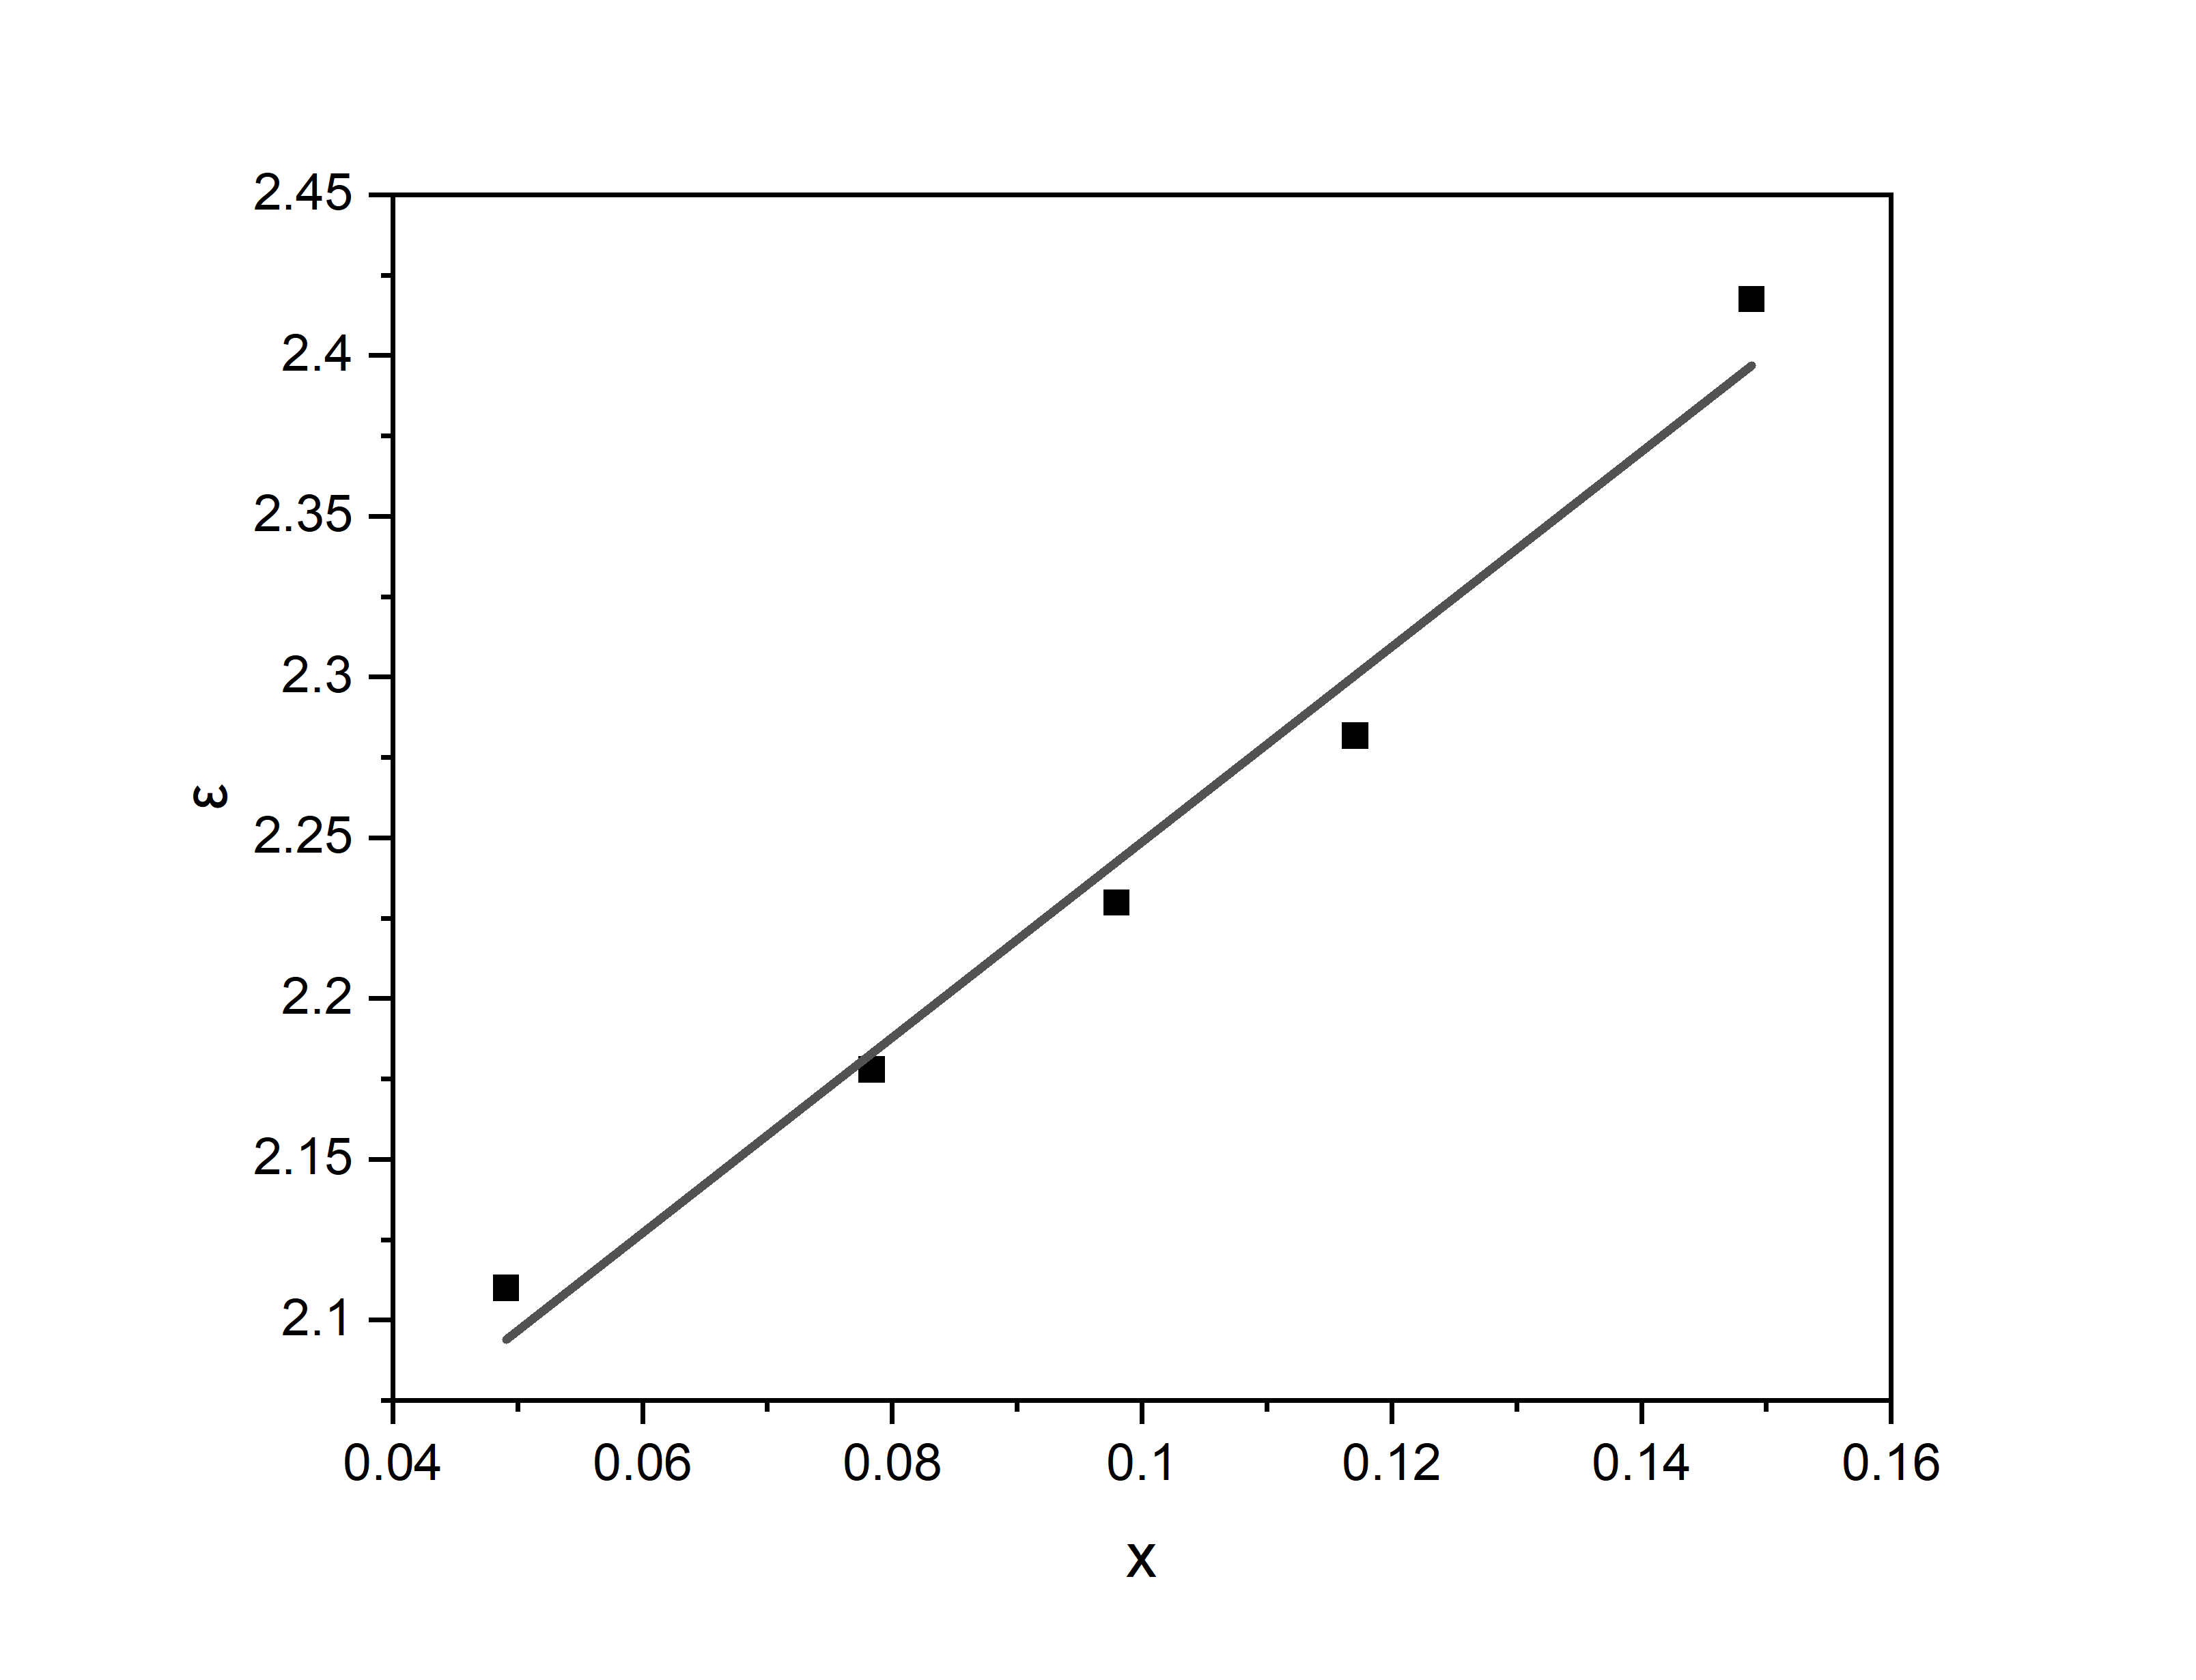
\includegraphics[width = .70\textwidth]{image/Graph6.png}
    \caption{相对介电常数与浓度关系}\label{3}
\end{figure}

\begin{figure}[htbp]
    \centering
    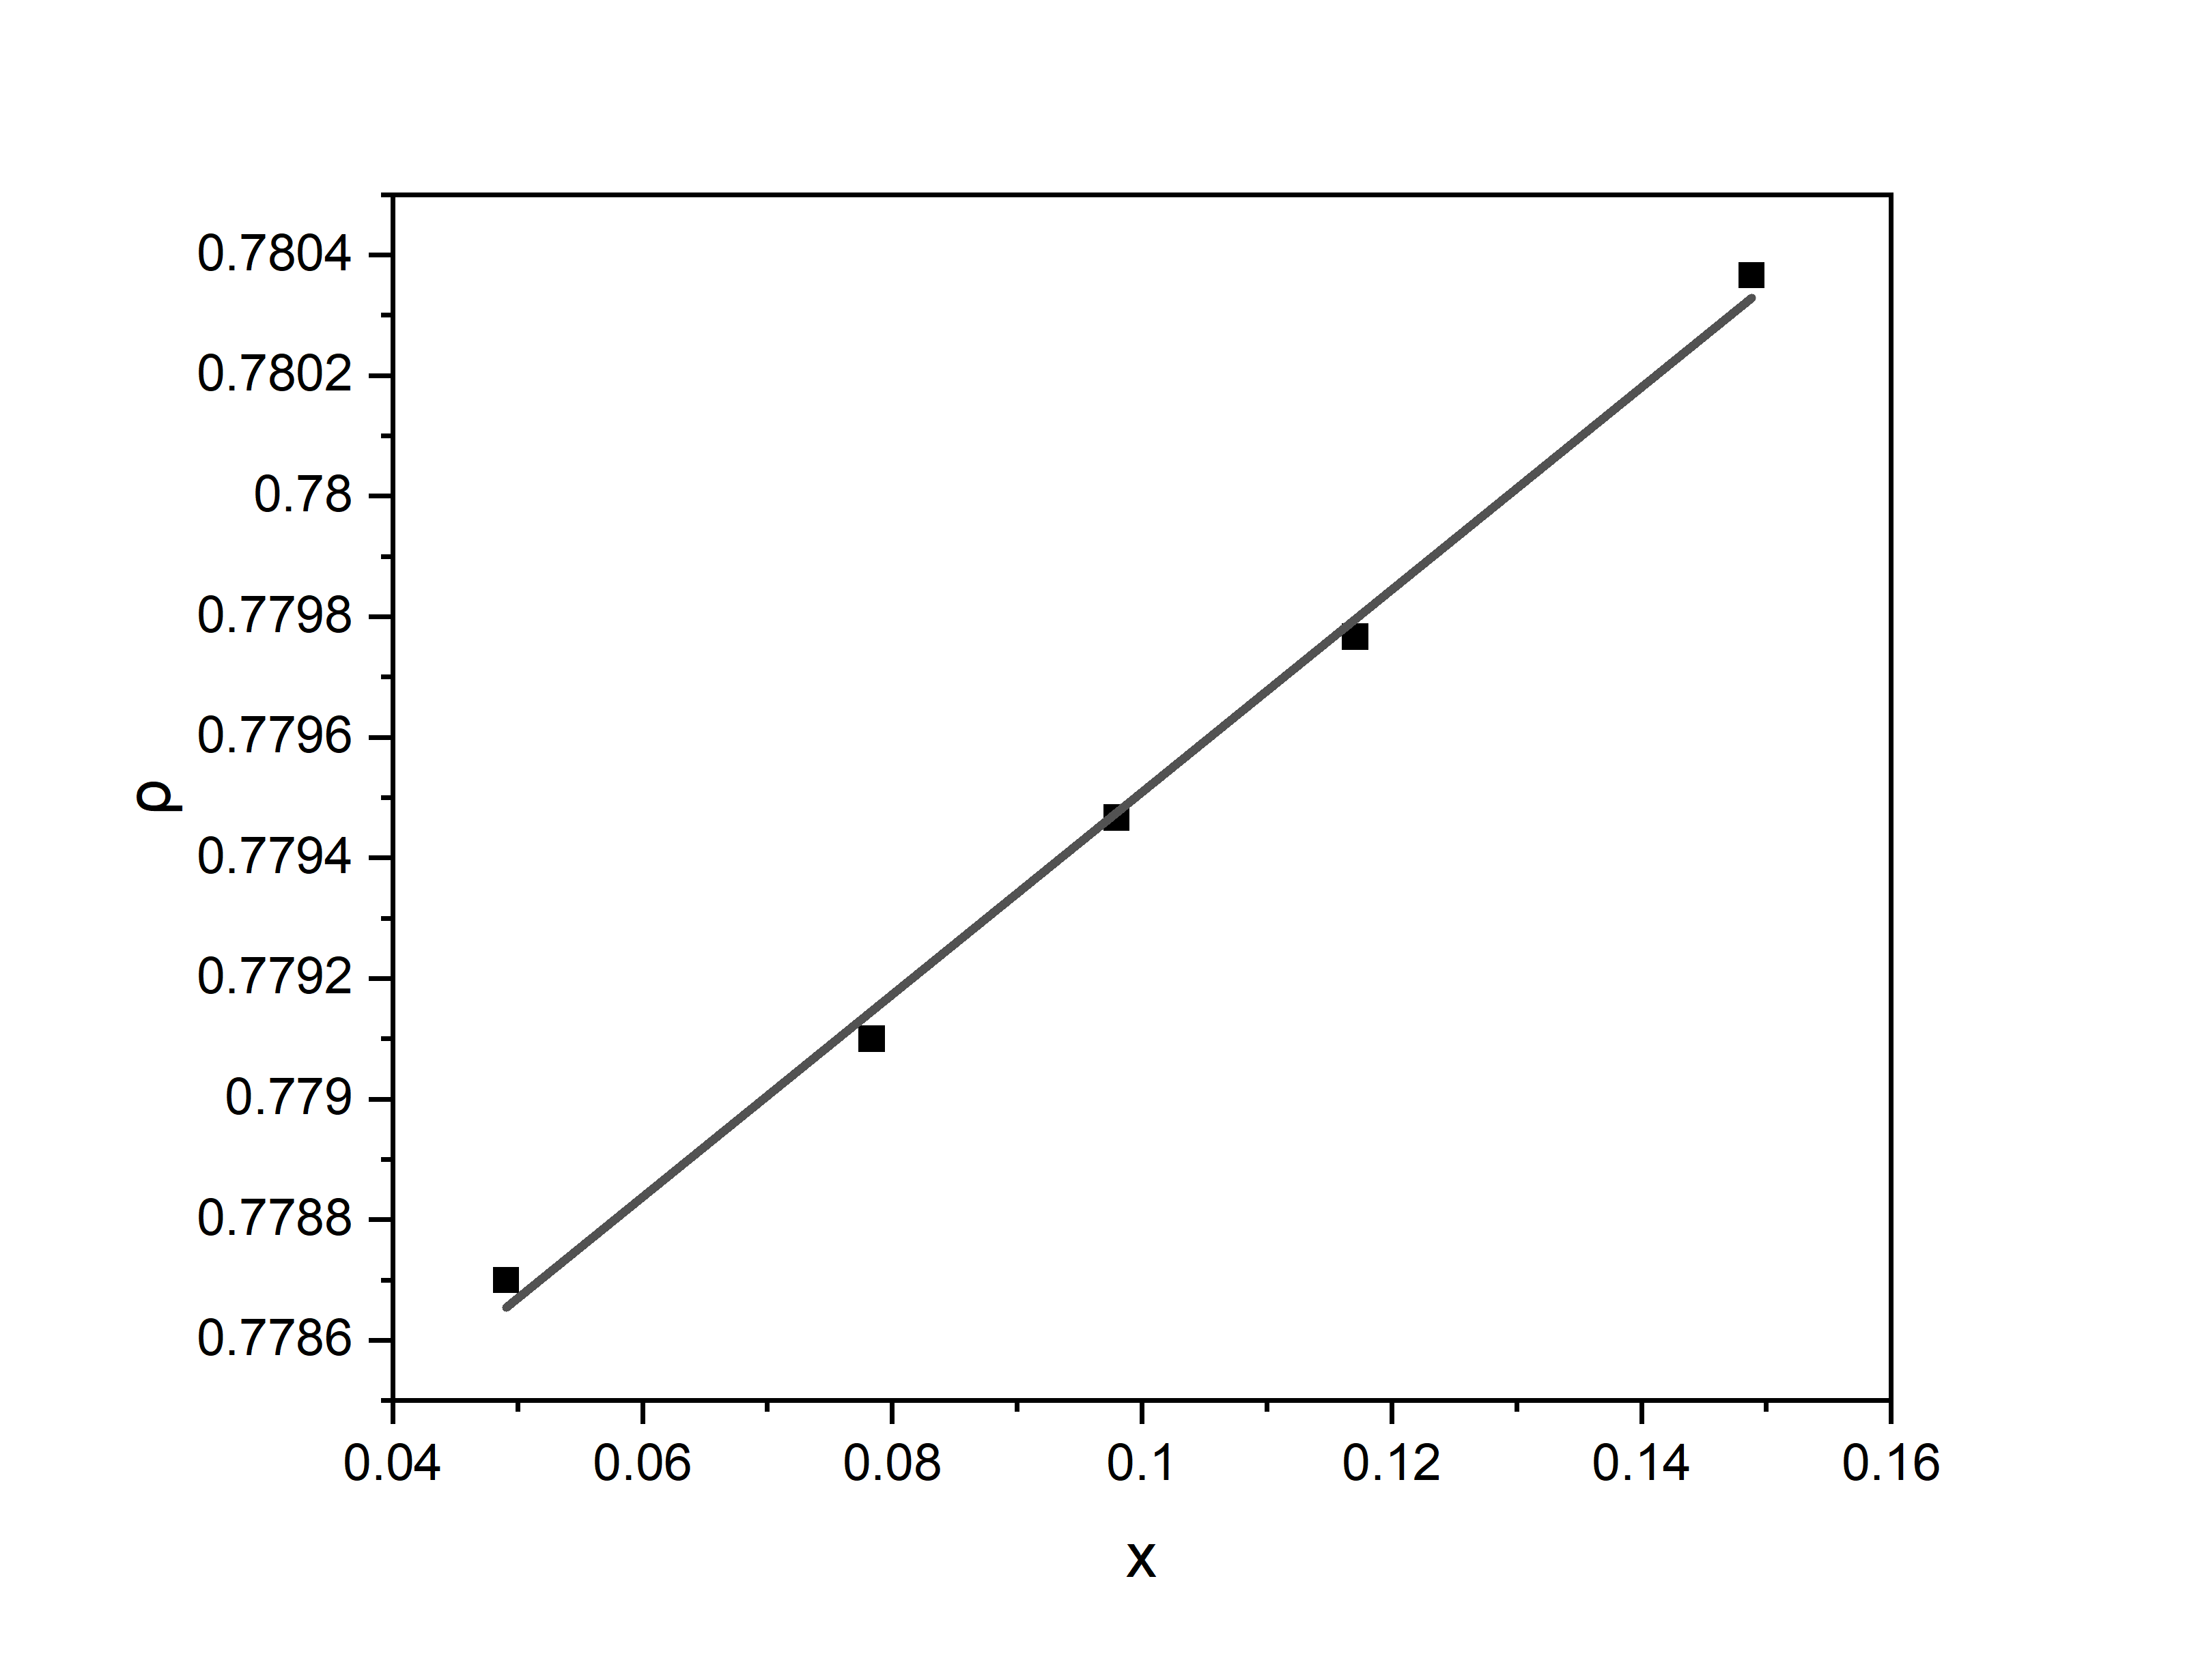
\includegraphics[width = .70\textwidth]{image/Graph3.png}
    \caption{密度与浓度关系}\label{4}
\end{figure}


由公式
\begin{equation}\label{002}
    \bar{P}_2^\infty = A (M_2 - b B) + a C
\end{equation}

其中
$$
A = \frac{\varepsilon_1 - 1}{\varepsilon_1 + 2}\times\frac{1}{\rho_1} = 3.06 \times 10^{-4} m^3/kg
$$
$$
B = \frac{M_1}{\rho_1} =  1.082 \times 10^{-4} m^3/mol
$$
$$
C = \frac{3M_1}{(\varepsilon_1 + 2)^2\rho_1} = 2.09 \times 10^{-5}
$$

因此代入公式 \ref{002} ,
$$
\bar{P}_2^\infty = A (M_2 - b B) + a C = 8.48 \times 10^{-5}m^3/mol
$$

得到$\bar{P}_2^\infty$ 为 $8.48 \times 10^{-5}m^3/mol$,由公式
\begin{equation}\label{003}
    \mu = 12.81\sqrt{(\bar{P}_2^\infty - R)T} = 1.72 D
\end{equation}

得到正丁醇的偶极矩为 1.72 D。由文献\cite{CRC},正丁醇的偶极矩为 1.66 D,实验值与理论值有一定偏差,误差分析详见讨论部分。

\section{实验结果与讨论}
\subsection{讨论}
\subsubsection{误差分析}
实验中计算了正丁醇的折射度,计算其误差为
$$
R = \frac{n^2-1}{n^2+2}\times\frac{M}{\rho} = 2.2281 \times 10^{-5} m^2\cdot mol^{-1}
$$
$$
\sigma_R = \sqrt{(\sigma_n \frac{\partial R}{\partial n})^2+(\sigma_\rho \frac{\partial R}{\partial \rho})^2} = 7 \times 10^{-9} m^2\cdot mol^{-1}
$$

因此,我们得到正丁醇的折射度为 $(2.2281 \pm 0.0007) \times 10^{-5} m^2\cdot mol^{-1}$

计算 $\bar{P}_2^\infty$ 误差为
\begin{equation*}
    \begin{aligned}
        \sigma_{\bar{P}_2^\infty} &= \sqrt{(\sigma_a \frac{\partial \bar{P}_2^\infty}{\partial a})^2+(\sigma_b \frac{\partial \bar{P}_2^\infty}{\partial b})^2+(\sigma_{\varepsilon_1} \frac{\partial \bar{P}_2^\infty}{\partial \varepsilon_1})^2+(\sigma_{\rho_1} \frac{\partial \bar{P}_2^\infty}{\partial \rho_1})^2} \\
                                  &= \sqrt{(\sigma_a C)^2+(\sigma_b AB)^2+(\sigma_{\varepsilon_1} \frac{\partial \bar{P}_2^\infty}{\partial \varepsilon_1})^2+(\sigma_{\rho_1} \frac{\partial \bar{P}_2^\infty}{\partial \rho_1})^2}
    \end{aligned}
\end{equation*}
$$
\sigma_{\varepsilon_1} = 0.03 \quad \sigma_a =  0.3
$$
$$
\sigma_{\rho_1} = 0.00006 kg/m^3 \quad \sigma_b = 0.0006 kg/m^3
$$
$$
\sigma_{\bar{P}_2^\infty} = 6 \times 10^{-6} m^3/mol
$$
得到 $\bar{P}_2^\infty$ 为 $(8.5 \pm 0.6) \times 10^{-5}m^3/mol$

$$
\sigma_\mu = \sqrt{(\sigma_{\bar{P}_2^\infty} \frac{\partial \mu}{\partial \bar{P}_2^\infty})^2+(\sigma_R \frac{\partial \mu}{\partial R})^2} = 0.08 D
$$
因此偶极矩为 $(1.72 \pm 0.08) D$。

\subsection{误差讨论}

得到正丁醇的偶极矩为 $(1.72 \pm 0.08) D$。由文献\cite{CRC},正丁醇的偶极矩为 1.66 D,实验值的误差与偏差都很大,可能的原因如下
\begin{enumerate}
    \item 本实验在计算中忽略了原子极化率,在总摩尔极化率中原子极化率大概占 $5$ ~ $1̃5\%$,
    因此将引入较大的偏差,如果假设原子极化率占诱导极化率的 $5\%$,则偶极矩为
    $$
        \mu = 12.81\sqrt{(\bar{P}_2^\infty\times 0.9 - R)T} = 1.67 D
    $$
    这样修正与结果相近,但是原子极化率比例不易确定。
    \item 本实验在计算中认为溶液均为理想溶液。理想溶液近似仅对稀溶液成立
    但是本实验中摩尔分数最大为 0.15。因此会明显偏离理想溶液,在图 \ref{3} 与图 \ref{4} 中可以看出
    溶液在摩尔分数为 0.15 时在一定程度上偏离拟合直线。观察两条拟合曲线可以发现,
    拟合出来是接近二次曲线关系,这可能是溶液配制较浓导致的,因此,可以考虑将溶液的浓度梯度降低一
    些,可能会有更好的结果。
    \item 本次实验的主要误差来源为电容的测量误差。
    $$
    \sigma_{\varepsilon_1} = 0.03 \quad \sigma_a =  0.3
    $$
    造成误差的原因是计算得到的相对介电常数的线性关系不好。可能的原因是溶液配制较浓,偏离理想溶液
    以及精密电容测量仪本身的误差较大。测量时的吹风机使得溶剂蒸发带走热量,降低了温度,也会引入误差。
    \item 温度对实验的影响也较大,经过测量,实验室的室温为 18 $\rm \degree C$,若使用 D50 型数字密度计,测量时
    温度为 20 $\rm \degree C$。使用阿贝折射仪时,由于靠近门口,测量温度为 14 $\rm \degree C$。在进行不同实验步骤时,
    温度差异较大,都会给实验带来一定的误差。文献中给出的偶极矩值均为在 25 $\rm \degree C$ 下的结果,也会对精度造成影响。    
\end{enumerate}

\subsection{结论}

本实验通过稀溶液法测定正丁醇的偶极矩,利用 D50 型与 DE45 型数字密度仪和精密电容测量仪来
测定正丁醇溶液的密度和电容,从而求出其总摩尔极化度为 $(8.5 \pm 0.6) \times 10^{-5}m^3/mol$;
利用阿贝折射仪测定正丁醇的折射率,进而求出其电子极化度
也就是摩尔折射度为 $(2.2281 \pm 0.0007) \times 10^{-5} m^2\cdot mol^{-1}$。
进一步计算其偶极矩为 $(1.72 \pm 0.08) D$。通过对实验结果的误差
分析可知,实验的误差主要来自于电容的测量和实验的原理误差,可以通过减小
实验体系的浓度,维持实验温度为一定值,来提高偶极矩的测量准确性。

\newpage

\section{附录}
\begin{figure}[htbp]
    \centering
    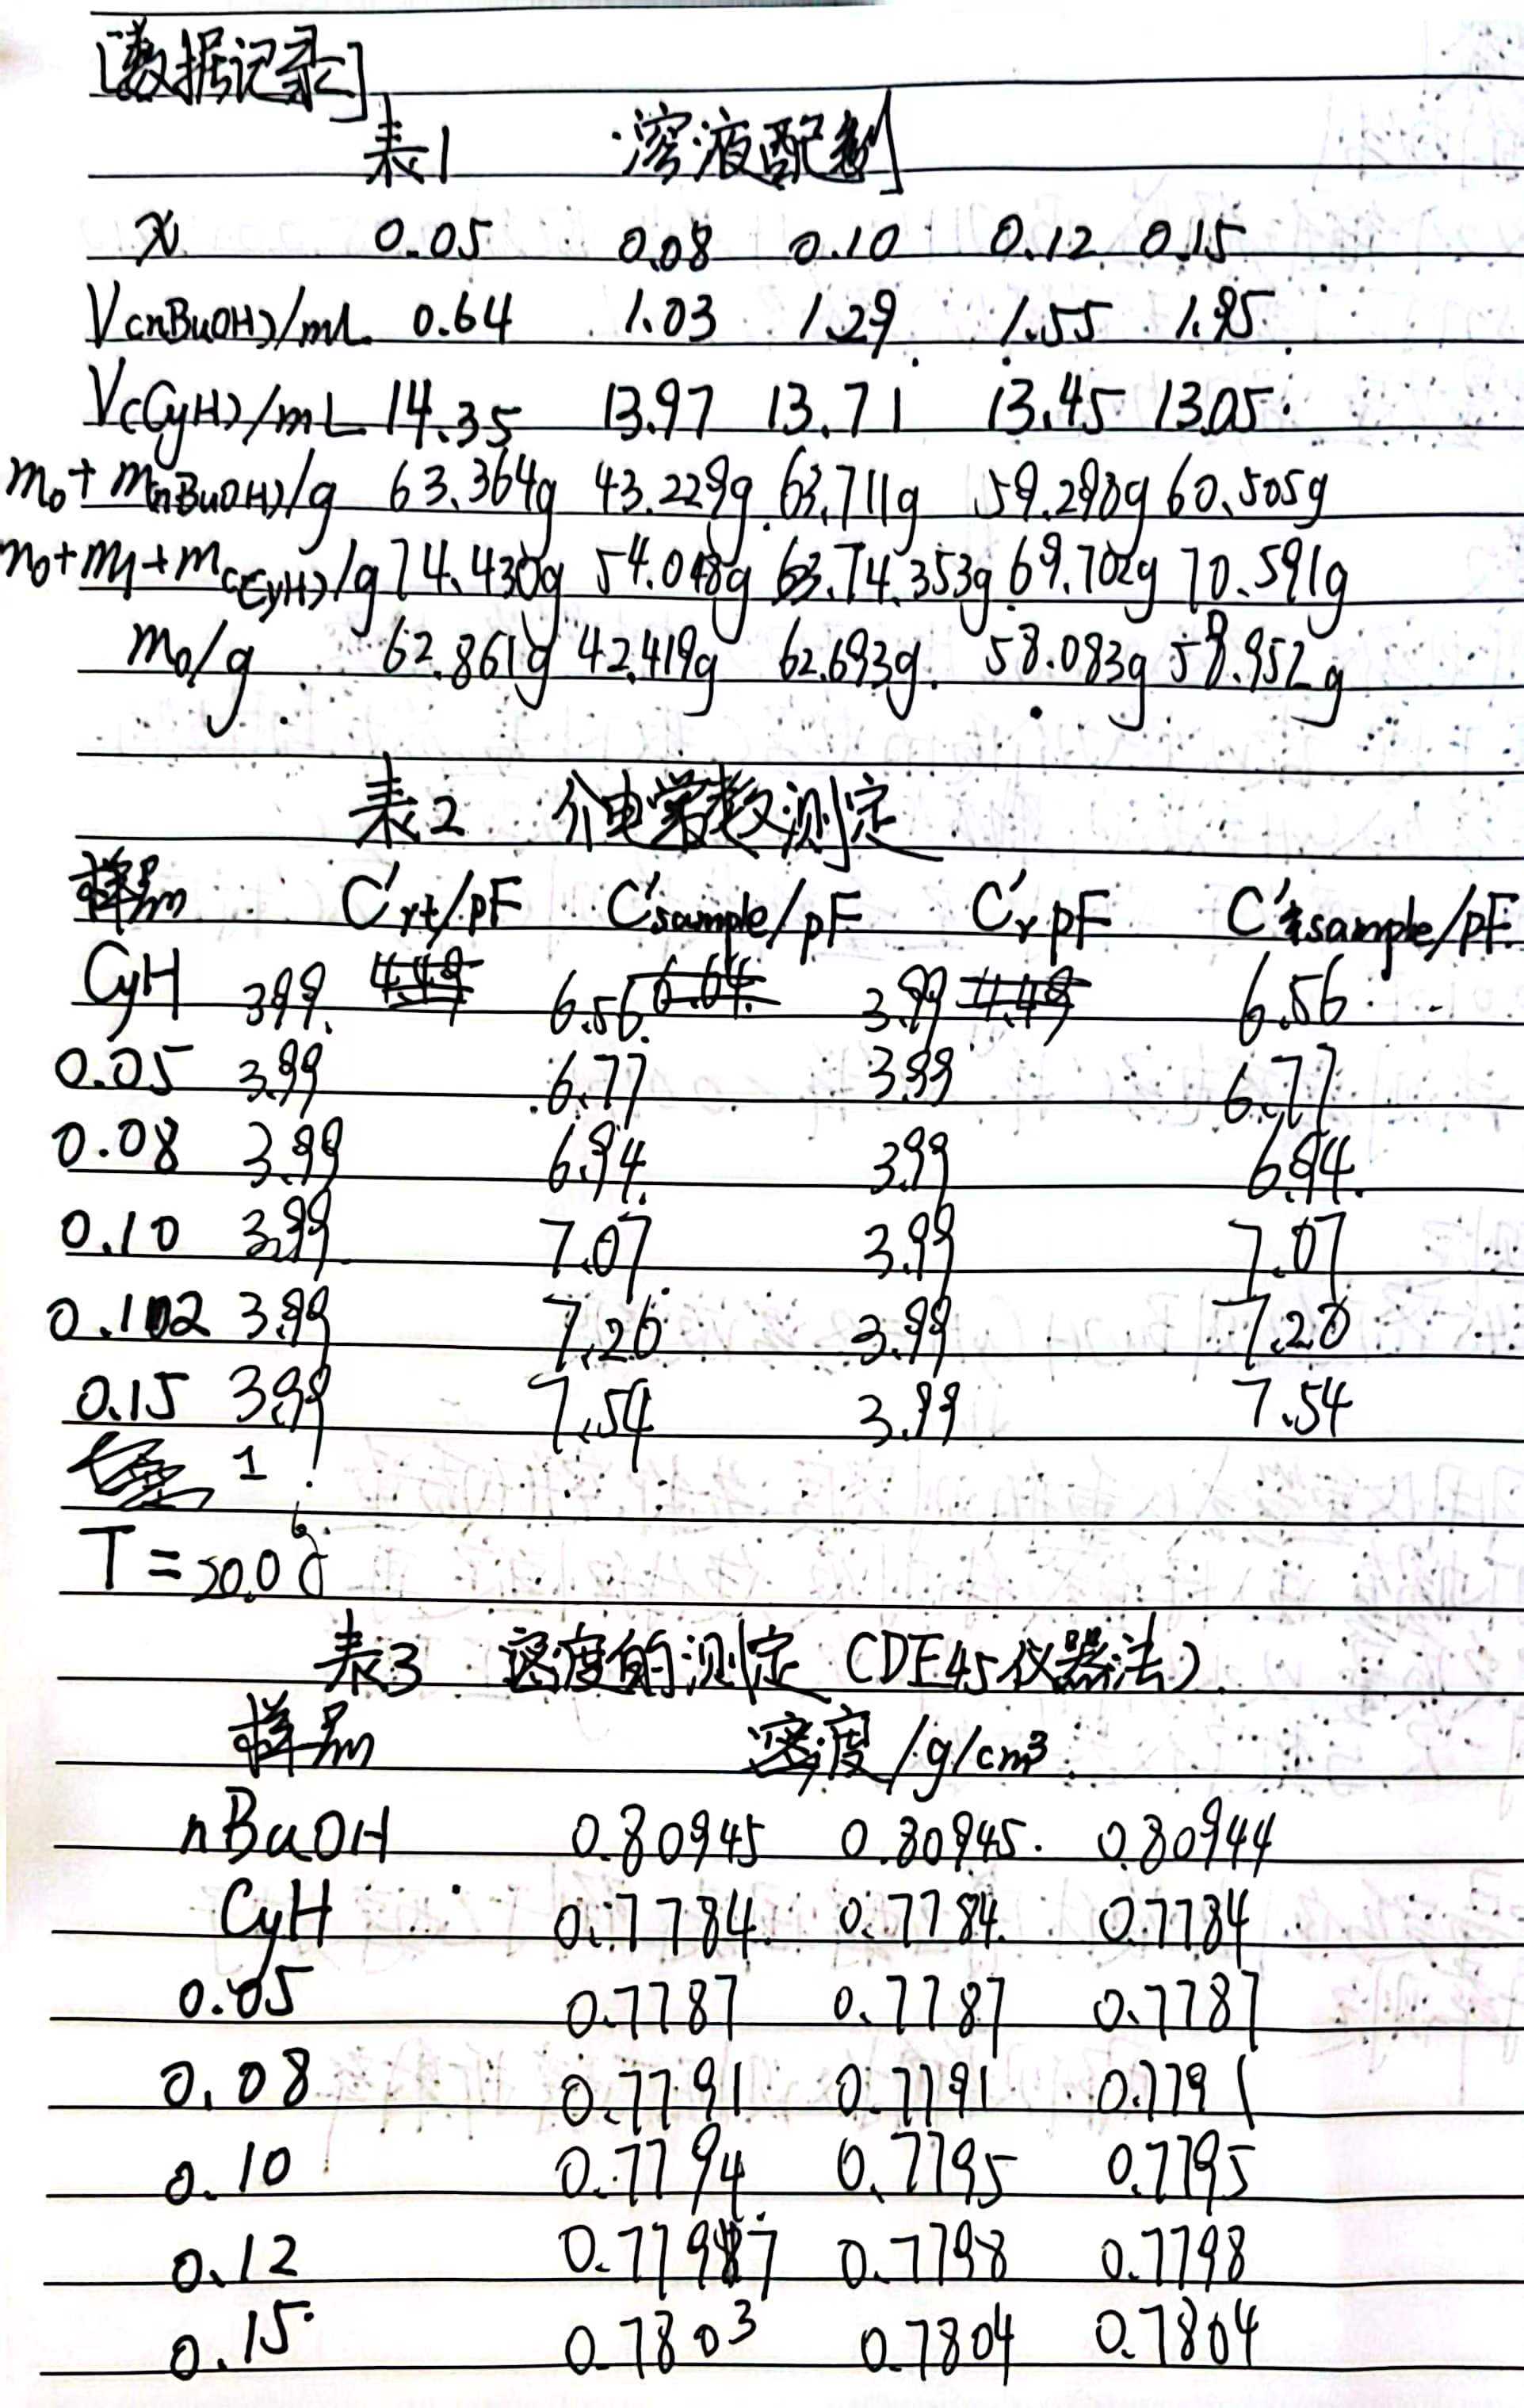
\includegraphics[width = .70\textwidth]{image/sysj.jpg}
    \caption{数据记录图片}\label{s0}
\end{figure}

\nocite{*}

\newpage
\bibliography{reference}
\end{document}
